
\documentclass[12pt]{article}

%Para algoritmos
\usepackage[ruled,linesnumbered,lined]{algorithm2e}
\usepackage{color}

\usepackage{sbc-template}

\usepackage{graphicx,url}

%Para o idioma português
\usepackage[brazil]{babel}   
\usepackage[utf8]{inputenc}  

     
\sloppy

\title{Escrevendo o seu texto científico em \LaTeX: 10 dicas básicas}

\author{Lesandro Ponciano\inst{1}}


\address{Departamento de Engenharia de Software e Sistemas de Informação\\  Pontifícia Universidade Católica de Minas Gerais (PUC Minas)\\
  Belo Horizonte -- MG -- Brasil
  \email{\{lesandrop\}@pucminas.br}
}

\hyphenation{a-ba-ca-te bo-la}
\begin{document} 

\maketitle

\begin{abstract}
  The two main goals of this short course are: 1) to present \LaTeX tips to students who do not yet know this language; and 2) introducing elements that are typical of being used in scientific paper in the computer area, such as equations, algorithms, tables, figures, and lists. As a method, this short course focuses on aspects of text composition rather than advanced topics on creating styling, templates and libraries.
\end{abstract}
     
\begin{resumo} 
  Os dois objetivo principais desta oficina são: 1) apresentar dicas de \LaTeX para alunos que ainda não conhecem essa linguagem; e 2) introduzir elementos que são típicos de serem usados em artigos científicos na área de informática, tais como equações, algoritmos, tabelas, figuras e listas. Como método, nesta oficina foca-se em aspectos da composição do texto em vez de tópicos avançados de criação de estilo, templates e bibliotecas.
\end{resumo}


\section{Edição online e \textit{Templates}}

Atualmente, há diversas plataformas online que permitem a edição de texto \LaTeX. Recomenda-se o uso da plataforma Overleaf~\footnote{URL: \url{https://www.overleaf.com/} Acesso em: 22/01/2020.}. Usar uma plataforma online evita o trabalho de instalar e configurar os diversos componentes de software que são necessários para usar o \LaTeX localmente.

Em suas tarefas como cientista, você raramente criará todo um documento \LaTeX. As conferências e periódicos geralmente disponibilizam um \textit{template} com o estilo de publicações. Trata-se de um documento de estilo, com todo formado padrão, que serve de exemplo na criação do artigo. Mesmo para atividades pessoas, há diversos templates disponíveis. O Overleaf mantém diversos templates~\footnote{URL: \url{https://www.overleaf.com/latex/templates} Acesso em: 22/01/2020.}. Usaremos o template para documentos no formato de conferências da  Sociedade Brasileira de Computação (SBC)~\footnote{URL: \url{https://www.overleaf.com/latex/templates/sbc-conferences-template/blbxwjwzdngr} Acesso em: 22/01/2020.}


\section{Formatação Textual Básica}

Vejamos itálico, negrito e aspas em Latex. Este é um texto normal. \textit{Este é um texto em itálico usando o comando textit.} {\it Este e um texto em itálico usando it}. Então, recapitulando:

Texto Normal.

\textit{Texto em itálico}.

{\it Texto em itálico}.

Não é muito diferente quando desejamos colocar um texto em negrito. Este é um texto normal. \textbf{Este é um texto em negrito usando o comando textbf.} {\bf Este e um texto em negrito usando bf}. Então, recapitulando:

Texto Normal.

\textbf{Texto em negrito}.

{\bf Texto em negrito}.

Em artigos científico em muitas situações desejamos colocar um termo ou fragmento de texto entre aspas (`` ''). Em \LaTeX há uma forma específica de fazer isso. Este é um texto com "aspas erradas". Este é um texto com ``aspas corretas''.


\section{Idioma e Separação Silábica}

Idioma é muito importante em \LaTeX. Ele define, por exemplo, a separação silábica. A depender do estilo, ele também determina o rótulo de figuras (se será \textit{Figure} ou Figura) e de tabelas (se será \textit{Table} ou Tabela)\ldots  Não confundir idioma do editor com idioma do documento!

Para colocar idioma em português use a biblioteca \textit{babel} no preâmbulo, da seguinte forma:\textcolor{blue}{\\usepackage[brazil]\{babel\}}. A fim de exemplo, essa biblioteca encontra-se adicionada neste documento.

Se mesmo com o idioma em português a separação silábica apresentar problemas, você forçá-la. Isso pode ser feito com o comando \textcolor{blue}{\\hyphenation\{a-ba-ca-te bo-la\}}.  Ele deve ser adicionando antes do início do documento.  A fim de exemplo, o hyphenation encontra-se adicionado neste documento.

\section{Listas}

Faça da seguinte forma:
\begin{enumerate}
    \item Acesse o \textit{template};
    \item Coloque o seu texto no \textit{template};
    \item Faça uma revisão cuidadosa;
    \item Envie ao orientador.
\end{enumerate}


Faça da seguinte forma:
\begin{itemize}
    \item Acesse o \textit{template};
    \item Coloque o seu texto no \textit{template};
    \item Faça uma revisão cuidadosa;
    \item Envie ao orientador.
\end{itemize}

\section{Equações}

É muito comum o uso equações em texto científico na área de Ciências Exatas e Informática. É importante distinguir se a equação parece como parte do texto (dentro do parágrafo) ou se ela aparece como um elemento a parte, numerada e referenciada no texto. Veja abaixo um exemplo empregando os dois casos. Observe que equação é referenciada no texto pelo seu \textit{label}, que é convertido em um número gerado automaticamente pelo \LaTeX.

A Equação~\ref{eq:baskara} é conhecida como Bhaskara. Ela apresenta uma solução para uma equação do segundo grau no formato $ax^2+bx+c=0$, para $a\neq 0$. Nessa equação, $\Delta = b^2-4ac$.

\begin{equation}
\label{eq:baskara}
  x=\frac{-b\pm\sqrt{\Delta}}{2a}
\end{equation} 


\section{Tabelas}

Tabelas são importantes na organização de materiais e métodos e na apresentação de resultados que envolvem diversas variáveis. São amplamente usadas na área de Ciências Exatas e Informática. Veja abaixo um exemplo de tabela. Observe que a tabela é referenciada no texto pelo seu \textit{label}, que é convertido em um número gerado automaticamente pelo \LaTeX. Este exemplo foi extraído do artigo \textit{Characterising volunteers' task execution patterns across projects on multi-project citizen science platforms}\cite{Ponciano:IHC:2019}.

Mostra-se importante analisar como as plataformas diferem entre si em termos de atenção recebida dos voluntários que contribuem nos projetos. A Tabela~\ref{tab:ineq} mostra  a inequalidade em cada plataforma. 

\begin{table}[htb]
  \caption{Comparação de Plataformas em termos de inequalidade (\textit{Gini coefficient}). Quanto mais próximo de 1, maior a inequalidade.}
  \centering
  \label{tab:ineq}
  \begin{tabular}{l|r|r}
  \hline
    Plataforma&Inequalidade no recrutamento&Inequalidade na contribuição recebida\\
    \hline
    Crowdcrafting      &  0.93 & 0.95\\
    GeoTag-X       &  0.47 & 0.64\\
    Socientize    &  0.61    & 0.80\\
  \hline
\end{tabular}
\end{table}

\section{Figuras}

Figuras são importantes na apresentação de resultados em artigos científicos. São amplamente usados na área de Ciências Exatas e Informática. Veja abaixo um exemplo de figura. Observe que a figura é referenciada no texto pelo seu \textit{label}, que é convertido em um número gerado automaticamente pelo \LaTeX. Este exemplo foi extraído da dissertação de mestrado \textit{Avaliação do impacto de estratégias de economia de energia em grades computacionais entre-pares}~\cite{Ponciano:Thesis:2011}

Podemos observar, pela Figura~\ref{fig:TimesTransition}, que não há evidências estatísticas de que as estratégias de dormência Sobreaviso e Hibernação apresentem impactos diferentes no número de transições realizadas pelas máquinas.

\begin{figure}[htb]
 \centering
 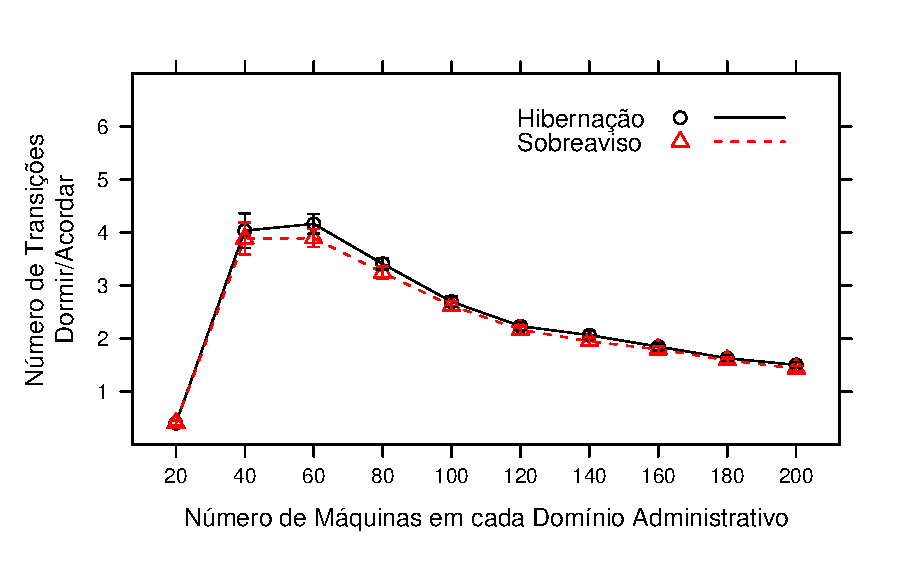
\includegraphics[width=0.9\linewidth]{TimesTransition.pdf}
 \caption{Número de transições dormir/acordar realizadas por cada máquina quando são utilizadas as estratégias de dormência Sobreaviso e Hibernação. Os domínios administrativos utilizam a estratégia de escolha MRS e TI definido como $0$.}
 \label{fig:TimesTransition}
\end{figure}

\section{Algoritmos}

O uso de algoritmo é muito frequente na área de Informática. Há diversos recursos que podem ser usados na confecção de algoritmos. O Algoritmo~\ref{alg:replication} é um exemplo de algoritmo feito usando a biblioteca \textit{algorithm2e}. Este exemplo foi extraído do artigo científico \textit{Agreement-based credibility assessment and task replication in human computation systems}~\cite{Ponciano:FGCS:2018}.

\newcommand\mycommfont[1]{\footnotesize\ttfamily\textcolor{blue}{#1}}
\SetCommentSty{mycommfont}

\begin{algorithm}[htb]
\SetAlgoNoLine
\SetKwInOut{Input}{input}\SetKwInOut{Output}{output}
\Input{Task $t$, Credibility metric $m$, Required credibility $reqCred$, Maximum number of replicas $maxRepl$, Urgency $urge$}
\Output{Final answer to the task $finalAnswer$, Credibility of the final answer $finalCred$\;}
\BlankLine
$countRepl\leftarrow0$\tcc*[r]{The total number of replicas already generated by the algorithm.}
$S_t\leftarrow \{\}$\tcc*[r]{Map of works who provides each answer.}
$numReplPerTurn \leftarrow max(\lfloor maxRepl \times urge \rfloor,1)$\;
\Repeat{$finalCred \geq reqCred$ or $countRepl = maxRepl$}{
                $numRepl \leftarrow min(numReplPerTurn,maxRepl-countRepl)$\;
                $createReplicas(numRepl,t,S_t)$\tcc*[r]{It creates $numRepl$ replicas of task $t$, waits for their answers, and stores these answers and respective worker ids in the map $S_t$.}
                $G\leftarrow computeWorkersCredibility(S_t,m)$\tcc*[r]{It computes the credibilities of workers using credibility metric $m$; the initial credibility of a worker is set to 0.51.}
                $finalAnswer, finalCred\leftarrow getTheMostCredibleGroupOfAnswer(G)$\tcc*[r]{It computes the credibilities of groups of answers using Equation 1.}
                $countRepl \leftarrow countRepl + numRepl$\;
}
\Return $finalAnswer, finalCred$\;
\caption{Credibility-based Task Replication}
\label{alg:replication}
\end{algorithm}


\section{Bibtex}

Veja o arquivo \textit{mybibfile.bib}.

\section{Citações no texto}

Como pode-se observar, a Knuth escreveu um livro acadêmico~\cite{knuth:84} e Ponciano et al. escreveram um artigo científico~\cite{Ponciano:CiSE:2014}.

\bibliographystyle{sbc}
\bibliography{mybibfile}

\end{document}